%!TEX root = ../../main.tex

\chapter{Spinners}
\label{cha:spinners}

\todo[inline]{\textbf{Describe Spinners (GirafSpinner):} This is also known as a dropdown menu. Describe how this should look like, and describe how to inser text into it. Create an appendix that describes how one uses GirafSpinner and GirafSpinnerAdapter. The spinner is not well implemented, but some soloution already exist called a GirafSpinner}

\begin{figure}[h]
	\centering
	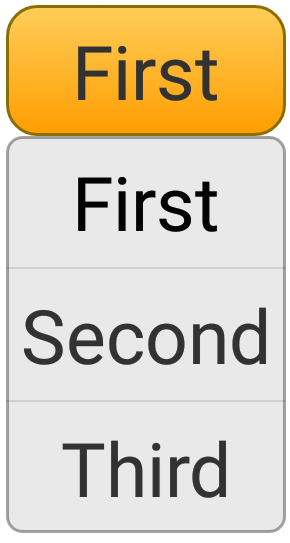
\includegraphics[width=0.1\textwidth]{girafspinner}
	\caption{Current implementation \androidinline{GirafSpinner}}
	\label{fig:girafspinner}
\end{figure}